% !TeX program = lualatex
% !TeX encoding = utf8
% !TeX spellcheck = uk_UA
% !BIB program = bibler

\documentclass{beamer}
\usetheme{Electromagnetism}
\usepackage{Electromagnetism}
%============================================================================
\title[Лекції електрики та магнетизму]{\huge\bfseries Енергія магнітного поля}
\subtitle{Лекції з квантової хімії}
\author{Пономаренко С. М.}
%============================================================================
\graphicspath{{pictures/}}
\begin{document}
\begin{frame}[plain]
	\maketitle
\end{frame}

%\begin{frame}{Енергія магнітного поля}
%\begin{block}{Магнітне поле}
%    Магнітне поле --- вид матерії, який несе в собі енергію. Задача --- знайти вираз для цієї енергії
%\end{block}
%\end{frame}

% ============================== Слайд ## ===================================
\begin{frame}{Явище самоіндукції}

	ЕРС у контурі виникає за будь-якої зміни магнітного потоку через його площу, незалежно від причини цієї зміни:
	\begin{equation*}
		\mathcal{E}_\text{ind} = -\frac1c \frac{d\Phi}{dt}
	\end{equation*}


		\begin{block}{Явище самоіндукції}
			Змінний магнітний потік може викликатись змінним струмом самого контуру. У цьому випадку в контурі також з'являється ЕРС --- вона називається електрорушійною силою самоіндукції.
		\end{block}

		\begin{center}
			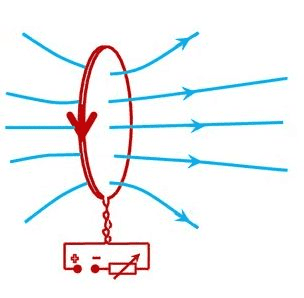
\includegraphics[width=0.35\linewidth]{selfinduction}
		\end{center}

\end{frame}
% ===========================================================================




% ============================== Слайд ## ===================================
\begin{frame}{Явище самоіндукції}{Індуктивність}
	Якщо електричний струм від зовнішнього джерела тече через контур, то навколишньому просторі виникає магнітне поле. У свою чергу, це поле створює магнітний потік, величина якого пропорційна силі струму:
	\begin{equation*}
		\Phi = \frac{L}{c} I
	\end{equation*}

	Коефіцієнт пропорційності $ L $ називається \emph{коефіцієнтом самоіндукції}, або \emph{індуктивністю} контуру. Він, подібно до ємності конденсатора,
	залежить від геометричної форми контуру та магнітної проникності навколишнього середовища.

	Для довгого соленоїда, що має $ N $ витків, довжину $ l $ та площу перерізу $ S $, і в середині якого вміщене осердя магнітною проникністю $ \mu $, індуктивність дорівнює:
	\begin{equation*}
		L = \frac{4\pi\mu N^2 S}{l}, \quad [L] = \text{см (в СГС)}.
	\end{equation*}

\end{frame}
% ===========================================================================




% ============================== Слайд ## ===================================
\begin{frame}{Явища при замиканні та розмиканні кіл}
	Якщо спробувати змінити силу струму, то в колі з'явиться ЕРС  самоіндукції, пропорційна швидкості зміни сили струму. ЕРС самоіндукції спрямована таким чином, щоб перешкодити зміні струму:
	\begin{equation*}
		\mathcal{E}_\text{si} = - \frac{L}{c^2}\frac{dI}{dt}.
	\end{equation*}
	\begin{center}
		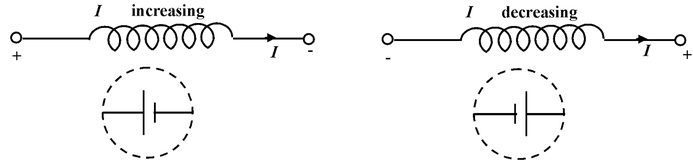
\includegraphics[width=0.75\linewidth]{addsource}
	\end{center}

	Закон Ома для кіл з індуктивністю:
	\begin{equation*}
		I = \frac{\mathcal{E} + \mathcal{E}_\text{si}}{R},
	\end{equation*}
	звідки
	\begin{equation*}
		\mathcal{E} = - \mathcal{E}_\text{si} + IR
	\end{equation*}
\end{frame}
% ===========================================================================





% ============================== Слайд ## ===================================
\begin{frame}{Енергія магнітного поля}{}

	Розглянемо ізольований контур. Контур нерухомий.

	Закон Ома:
	\begin{equation*}
		\mathcal{E} = - \mathcal{E}_\text{si} + IR \quad / \quad \cdot dq = I dt
	\end{equation*}

	\begin{equation*}
		\underbrace{\mathcal{E} I dt}_{\text{Робота джерела}} = \underbrace{d \left(  \frac{LI^2}{2c^2}\right)}_{\text{Зміна енергії магнітного поля}}  + \underbrace{I^2Rdt}_{\text{Теплота}}
	\end{equation*}

	\begin{alertblock}{}
		Робота джерела частково розсіюється у вигляді теплоти і частково йде на утворення магнітного поля.
	\end{alertblock}

	\begin{equation*}
		W_m = \frac{LI^2}{2c^2} = \frac{\Phi^2}{2L} = \frac{I\Phi}{2c}.
	\end{equation*}
\end{frame}
% ===========================================================================





% ============================== Слайд ## ===================================
\begin{frame}{Локалізація енергії магнітного поля. Густина енергії}{}
	Вираз для магнітної енергії можна перетворити на іншу форму, яка відповідає
	зовсім іншому уявленню про місце знаходження енергії.


	\bigskip

	{\scriptsize

		Покажемо це на прикладі довгого соленоїда. Для соленоїда потік власного магнітного поля $ \Phi = NBS $, індуктивність --- $ L =  \frac{4\pi\mu N^2 S}{l}$, отже

		\begin{equation*}
			W_m = \frac{\Phi^2}{2L} = \frac{N^2 B^2 S^2}{2} \frac{l}{4\pi\mu N^2 S} = \frac{B^2}{8\pi\mu} V = \frac{BH}{8\pi} V .
		\end{equation*}
	}
	В загальному випадку:
	\begin{equation*}
		W_m = \iiint\limits_V  \frac{\vect{B}\cdot\vect{H}}{8\pi} dV = \iiint\limits_V w_m dV,  \quad w_m = \frac{\vect{B}\cdot\vect{H}}{8\pi}
	\end{equation*}
	де $ w_m $ --- густина енергії магнітного поля.

	\begin{alertblock}{}
		Магнітна енергія локалізована у просторі з об'ємною густиною  $ w_m $. Це відповідає уявленням теорії поля.
	\end{alertblock}
\end{frame}
% ===========================================================================



% ============================== Слайд ## ===================================
\begin{frame}{Явище взаємоіндукції}

	ЕРС у контурі виникає за будь-якої зміни магнітного потоку через його площу, незалежно від причини цієї зміни:
	\begin{equation*}
		\mathcal{E}_\text{ind} = -\frac1c \frac{d\Phi}{dt}
	\end{equation*}



	\begin{block}{Явище взаємоіндукції}
		Змінний струм, що протікає в одному з контурів, наприклад, у контурі $ 1 $, створює змінне магнітне поле, яке викликає появу $ ЕРС $ індукції у провідному контурі $ 2 $. Таке явище називається \emph{взаємною індукцією}.
	\end{block}

	\begin{center}
		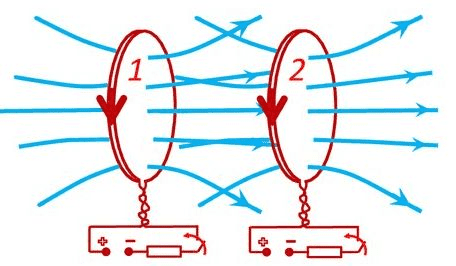
\includegraphics[width=0.5\linewidth]{interinduction}
	\end{center}
\end{frame}
% ===========================================================================



% ============================== Слайд ## ===================================
\begin{frame}{Коефіцієнти взаємної індукції}{}
	\begin{center}
		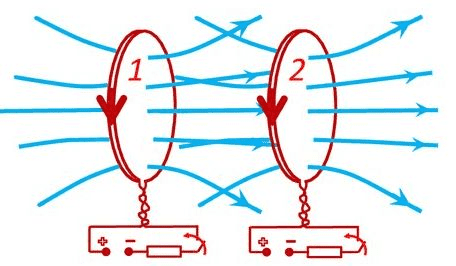
\includegraphics[width=0.5\linewidth]{interinduction}
	\end{center}

    Потоки через контури:
    \begin{equation*}
    \begin{cases}
        \Phi_1  = \frac{L_{11}}{c} I_1 + \frac{L_{12}}{c} I_2, \\[1ex]
        \Phi_2  = \frac{L_{21}}{c} I_1 + \frac{L_{22}}{c} I_2.
    \end{cases}
    \end{equation*}

    Коефіцієнти $ L_{11} $ і $ L_{22} $ є \emph{індуктивностями} відповідних контурів.

    Коефіцієнти $ L_{12} $ і $ L_{21} $ називаються \emph{коефіцієнтами взаємної індукції}. Вони характеризують магнітний зв'язок між контурами. У вакуумі коефіцієнти залежать від форми контурів та їхнього взаємного розташування.

\end{frame}
% ===========================================================================




% ============================== Слайд ## ===================================
\begin{frame}{Теорема взаємності}{}
	\tikz[remember picture,overlay] \node[inner sep=0pt, anchor=north east] at ([shift={(-0.5, -2)}]current page.north east){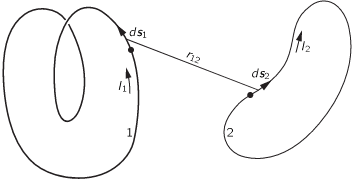
\includegraphics[width=4cm]{coeffinterinduction}};

Коефіцієнти взаємної індукції дорівнюють:
       \begin{equation*}
           \tcbhighmath{L_{12} = L_{21}}.
       \end{equation*}

       Взаємні потоки $ \Phi_{21}  =  \frac{1}{c} L_{21} I_1 = \iint\limits_{S_2} \Bfield_1 \cdot d\vect{S}_2 $, $ \Phi_{12}  = \frac{1}{c} L_{12} I_2 =  \iint\limits_{S_1} \Bfield_2 \cdot d\vect{S}_1 $.

       \medskip

       \begin{equation*}
           \Phi_{21}  = \iint\limits_{S_2} \Bfield_1 \cdot d\vect{S}_2 = \iint\limits_{S_2} \rot\vect{A}_1 \cdot d\vect{S}_2 = \oint\limits_{L_1} \vect{A}_1 \cdot d\vect{l}_2 = \frac1c \oint\limits_{L_1} \frac{ d\vect{l}_1 d\vect{l}_2 }{r_{12}} I_1,
       \end{equation*}
       звідки
       \begin{equation*}
           L_{21} = \oint\limits_{L_1} \frac{ d\vect{l}_1 d\vect{l}_2 }{r_{12}}.
       \end{equation*}

\end{frame}
% ===========================================================================




% ============================== Слайд ## ===================================
\begin{frame}{Енергія магнітного поля в загальному вигляді}{}\small
       При зміні струму $ I_1 $ у другому $ 2 $ контурі виникне ЕРС, що дорівнює:
       \begin{equation*}
           \mathcal{E}_2 = -\frac{d\Phi_{21}}{dt} = -\frac1{c^2} L_{21}I_1
       \end{equation*}
      Аналогічно, при зміні струму $ I_2 $ у першому $ 1 $ контурі виникне ЕРС, що дорівнює:
      \begin{equation*}
          \mathcal{E}_1 = -\frac{d\Phi_{12}}{dt} = -\frac1{c^2} L_{12}I_2
      \end{equation*}

     Вся робота, що виконується джерелами (за винятком джоулевої теплоти) за час $ dt $ проти   $ \mathcal{E}_\text{ind} $ і йде на зміну магнітної енергії:

\begin{overprint}
\onslide<1>
     \begin{multline*}
     \delta (A - Q) = \overbrace{- \mathcal{E}^\text{ind}_1 I_1 dt -  \mathcal{E}^\text{ind}_2 I_2 dt}^{dW_m} =  \\
      = \frac1{c^2} (L_{11} I_1 dI_1 + L_{12} I_1 dI_2 +  L_{21} I_2 dI_1 + L_{22} I_2 dI_1 ) = \\
      = d \left(  \frac{L_{11} I_1^2}{2c^2} + \frac{L_{22} I_2^2}{2c^2} + L_{12} I_1I_2\right) .
     \end{multline*}
     \onslide<2>
     В загальному вигляді
     \begin{equation*}
     W_m = \frac{1}{2c^2}\sum\limits_i\sum\limits_j L_ij I_i I_j.
     \end{equation*}

     Через поле (у вакуумі) $ \Bfield = \Bfield_1 + \Bfield_2 $
     \begin{equation*}
     W_m = \iiint\limits_V \frac{(\Bfield_1 + \Bfield_2)^2}{8\pi} dV = \iiint\limits_V \frac{B_1^2}{8\pi} dV + \iiint\limits_V \frac{B_2^2}{8\pi} dV + \iiint\limits_V \frac{\Bfield_1\cdot\Bfield_2}{4\pi} dV
     \end{equation*}
\end{overprint}

\end{frame}
% ===========================================================================





% ============================== Слайд ## ===================================
\begin{frame}{Обчислення сил з виразу для енергії}{}
	Розглянемо випадок, коли робота джерела також йде на виконання механічної роботи:

\begin{equation*}
    \mathcal{E} I dt - \delta Q = -\mathcal{E}_\text{ind} I dt =dW_m + \delta A_\text{мех}
\end{equation*}

\begin{equation*}
    \frac{I}{c} d\Phi = dW_m + \delta A_\text{мех}
\end{equation*}


\begin{overprint}
\onslide<1> Розглянемо віртуальні процеси, у яких зберігаються магнітні потоки $ d\Phi = 0 $, тоді:
\begin{equation*}
\delta A = -dW_m,
\end{equation*}

\begin{equation*}
\vect{F} = \frac{\delta A_\text{мех}}{d\vect{r}} = - \left( \frac{dW_m}{d\vect{r}}\right)_{\Phi = \const}
\end{equation*}
\onslide<2> Розглянемо віртуальні процеси, у яких зберігаються сили струму $ I = \const $. В такому випадку $ dW_m  = \frac1c \frac{I d\Phi}{2}$, отже $ \delta A_\text{мех} = + dW_m $, звідки

\begin{equation*}
\vect{F} = \frac{\delta A_\text{мех}}{d\vect{r}} = + \left( \frac{dW_m}{d\vect{r}}\right)_{I = \const}
\end{equation*}

\end{overprint}


\end{frame}
% ===========================================================================




% ============================== Слайд ## ===================================
\begin{frame}[t]{Приклади}{}
У центрі тонкої котушки радіусом, що містить $ N $ витків, знаходиться невеликий циліндричний магніт. Котушка підключена до балістичного гальванометра.
Опір кола $ R $. Після того, як магніт швидко видалили з котушки, через гальванометр пройшов заряд $ q $. Визначити магнітний момент магніту $ p_m $.
\end{frame}
% ===========================================================================



% ============================== Слайд ## ===================================
\begin{frame}[t]{Приклад}{}
       У соленоїд, площа кругового перерізу якого $ S $, довжина $ l $, що має $ n $ витків на одиницю довжини, всунутий магнетик з магнітною
       проникністю $ \mu $ на половину його довжини. Знайти силу, що діє на магнетик. По соленоїду йде струм $ I  $.
\end{frame}
% ===========================================================================





% ============================== Слайд ## ===================================
\begin{frame}[t]{Приклади}{}
Обчислити підйомну силу електромагніту з осердям з м'якого заліза.
\begin{flushright}
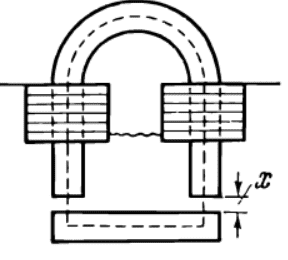
\includegraphics[width=0.5\linewidth]{magnet}
\end{flushright}
\end{frame}
% ===========================================================================

\end{document}
